When it comes to blackbox attacks, two existing approaches are evaluated: the Transfer based approach and the Boundary attack. In this section, results are only presented, but not discussed. The discussion is left for Section \ref{sec:discussion}.

In the transfer based approach, as described in Section \ref{sec:transfer-based}, the goal is to train a substitute network that will learn similar decision boundaries for every class as the targeted network. This implies that total number of possible classes should be the same, but an architecture of the substitute network may be different.

To get information about boundaries of the targeted neural network,  I take 778 samples that are previously unseen to targeted neural network, obtain labels for those samples and train a substitute neural network based on those results. Distribution of samples over age is presented in Figure \ref{fig:custom-dataset}.
 
 \begin{figure}[h]
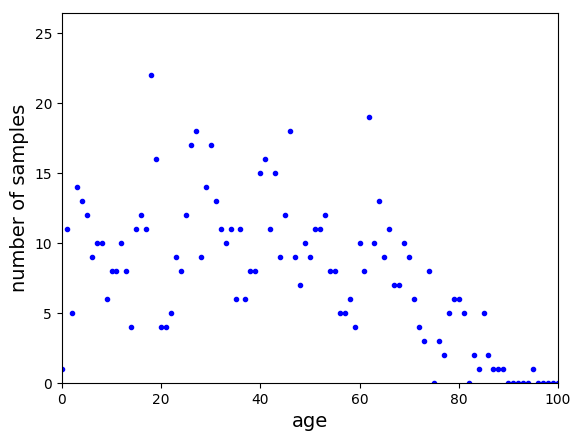
\includegraphics[width=13cm]{custom-dataset}
\caption{Number of samples per age in the dataset that is used for training a substitute neural network by querying a targeted blackbox neural network}
\label{fig:custom-dataset}
\end{figure}

Next, I take random 200 samples that are yet unseen by both networks and evaluate MAE of the targeted neural network and the substitute network on those 200 images. Then I craft adversarial samples for the substitute neural network using those 200 images. Target labels for adversarial samples are set in the same manner as in whitebox attacks, i.e. label 90 if a person is under 50 years old and label 10 if a person is over 50 years old. 

Finally, I evaluate MAE of the targeted neural network and the substitute network on the 200 adversarial samples crafted in the previous step.


In my first attempt, I tried to use the InceptionResNetV2 architecture as a substitute network. Since the targeted network has the same architectures, high number of adversarial samples that are transferred is expected. However, the experiment failed due to memory consumption when jacobian augmentation of the dataset is performed. 

In my second attempt, I used ResNet50 architecture for a substitute network instead of InceptionResNetV2 architecture. However, the experiment again failed  due to the memory exhaustion. 

In my third attempt, I used a vanilla CNN with three convolutional layers followed by flatten layer and softmax layer used for classification. However, the experiment failed due to the memory exhaustion.

Finally, since the goal is that a substitute neural network have similar boundaries for classification as the targeted neural network, those boundaries could be obtained to certain extent by just querying the targeted neural network and then learning the substitute neural network based on the results of queries. This approach skips a step of the jacobian augmentation of the dataset. Further argumentation of this decision can be found in Section \ref{sec:threats-to-validity}.

Results are presented in Tables
\ref{table:bbox-resnet50-sgd-fgsm},
\ref{table:bbox-resnet50-adam-fgsm}, 
\ref{table:bbox-resnet50-sgd-cw},
\ref{table:bbox-resnet50-adam-cw}, 
\ref{table:bbox-inception-sgd-fgsm},
\ref{table:bbox-inception-adam-fgsm}, 
\ref{table:bbox-inception-sgd-cw}, and
\ref{table:bbox-inception-adam-cw}.

% Please add the following required packages to your document preamble:
% \usepackage{graphicx}
\begin{table}[]
\resizebox{\textwidth}{!}{%
\begin{tabular}{|c|c|c|c|c|c|c|c|c|}
\hline
 & \multicolumn{2}{c|}{clean samples} & \multicolumn{6}{c|}{adversarial samples} \\ \hline
blackbox model id & blackbox MAE & substitute MAE & blackbox MAE & substitute MAE & avg L2 & std dev L2 & min L2 & max L2 \\ \hline
1 &  6.42 &  12.42 & 6.92 & 19.14  &  1890.86 & 58.77 &  1580.84 & 1939.89 \\ \hline
2 & 6.99 & 11.52 & 10.2 &  23.145 &  1891.01 & 59.07 & 1565.25 & 1939.89  \\ \hline
3 & 5.29 & 14.275 & 5.79  & 25.685 & 1891.34  & 58.79 & 1559.34 & 1939.89  \\ \hline
4 & TODO & TODO & TODO & TODO &  TODO & TODO & TODO &  \\ \hline
\end{tabular}%
}
\caption{Substitute network: ResNet50 architecture with SGD optimizer; Attack: FGSM}
\label{table:bbox-resnet50-sgd-fgsm}
\end{table}

% Please add the following required packages to your document preamble:
% \usepackage{graphicx}
\begin{table}[]
\resizebox{\textwidth}{!}{%
\begin{tabular}{|c|c|c|c|c|c|c|c|c|}
\hline
 & \multicolumn{2}{c|}{clean samples} & \multicolumn{6}{c|}{adversarial samples} \\ \hline
blackbox model id & blackbox MAE & substitute MAE & blackbox MAE & substitute MAE & avg L2 & std dev L2 & min L2 & max L2 \\ \hline
1 & 6.42 & 20.275 & 6.99 & 19.91  & 1890.10 & 60.31  &  1555.87 & 1939.89  \\ \hline
2 & 6.99 & 11.94 & 7.44 & 12.145 & 1921.91  &  21.20 &  1809.24 & 1939.89  \\ \hline
3 & 5.29 & 24.99 & 26.1 & 4.91 & 1893.30 & 58.41 & 1534.87 & 1939.89  \\ \hline
4 &  &  &  &  &  &  &  &  \\ \hline
\end{tabular}%
}
\caption{Substitute network: ResNet50 architecture with Adam optimizer; Attack: FGSM}
\label{table:bbox-resnet50-adam-fgsm}
\end{table}

% Please add the following required packages to your document preamble:
% \usepackage{graphicx}
\begin{table}[]
\resizebox{\textwidth}{!}{%
\begin{tabular}{|c|c|c|c|c|c|c|c|c|}
\hline
 & \multicolumn{2}{c|}{clean samples} & \multicolumn{6}{c|}{adversarial samples} \\ \hline
blackbox model id & blackbox MAE & substitute MAE & blackbox MAE & substitute MAE & avg L2 & std dev L2 & min L2 & max L2 \\ \hline
1 & 6.42 &  &  &  &  &  &  &  \\ \hline
2 & 6.99 &  &  &  &  &  &  &  \\ \hline
3 &  &  &  &  &  &  &  &  \\ \hline
4 &  &  &  &  &  &  &  &  \\ \hline
\end{tabular}%
}
\caption{Substitute network: ResNet50 architecture with Adam optimizer; Attack: CW}
\label{table:bbox-resnet50-sgd-cw}
\end{table}

% Please add the following required packages to your document preamble:
% \usepackage{graphicx}
\begin{table}[]
\resizebox{\textwidth}{!}{%
\begin{tabular}{|c|c|c|c|c|c|c|c|c|}
\hline
 & \multicolumn{2}{c|}{clean samples} & \multicolumn{6}{c|}{adversarial samples} \\ \hline
blackbox model id & blackbox MAE & substitute MAE & blackbox MAE & substitute MAE & avg L2 & std dev L2 & min L2 & max L2 \\ \hline
1 & 6.42 &  &  &  &  &  &  &  \\ \hline
2 & 6.99  &  &  &  &  &  &  &  \\ \hline
3 &  &  &  &  &  &  &  &  \\ \hline
4 &  &  &  &  &  &  &  &  \\ \hline
\end{tabular}%
}
\caption{Substitute network: ResNet50 architecture with Adam optimizer; Attack: CW}
\label{table:bbox-resnet50-adam-cw}
\end{table}

% Please add the following required packages to your document preamble:
% \usepackage{graphicx}
\begin{table}[]
\resizebox{\textwidth}{!}{%
\begin{tabular}{|c|c|c|c|c|c|c|c|c|}
\hline
 & \multicolumn{2}{c|}{clean samples} & \multicolumn{6}{c|}{adversarial samples} \\ \hline
blackbox model id & blackbox MAE & substitute MAE & blackbox MAE & substitute MAE & avg L2 & std dev L2 & min L2 & max L2 \\ \hline
1 & 6.42 &  &  &  &  &  &  &  \\ \hline
2 & 6.99  &  &  &  &  &  &  &  \\ \hline
3 &  &  &  &  &  &  &  &  \\ \hline
4 &  &  &  &  &  &  &  &  \\ \hline
\end{tabular}%
}
\caption{Substitute network: InceptionResNetV2 architecture with SGD optimizer; Attack: FGSM}
\label{table:bbox-inception-sgd-fgsm}
\end{table}

% Please add the following required packages to your document preamble:
% \usepackage{graphicx}
\begin{table}[]
\resizebox{\textwidth}{!}{%
\begin{tabular}{|c|c|c|c|c|c|c|c|c|}
\hline
 & \multicolumn{2}{c|}{clean samples} & \multicolumn{6}{c|}{adversarial samples} \\ \hline
blackbox model id & blackbox MAE & substitute MAE & blackbox MAE & substitute MAE & avg L2 & std dev L2 & min L2 & max L2 \\ \hline
1 & 6.42 &  &  &  &  &  &  &  \\ \hline
2 & 6.99 &  &  &  &  &  &  &  \\ \hline
3 &  &  &  &  &  &  &  &  \\ \hline
4 &  &  &  &  &  &  &  &  \\ \hline
\end{tabular}%
}
\caption{Substitute network: InceptionResNetV2 architecture with Adam optimizer; Attack: FGSM}
\label{table:bbox-inception-adam-fgsm}
\end{table}

% Please add the following required packages to your document preamble:
% \usepackage{graphicx}
\begin{table}[]
\resizebox{\textwidth}{!}{%
\begin{tabular}{|c|c|c|c|c|c|c|c|c|}
\hline
 & \multicolumn{2}{c|}{clean samples} & \multicolumn{6}{c|}{adversarial samples} \\ \hline
blackbox model id & blackbox MAE & substitute MAE & blackbox MAE & substitute MAE & avg L2 & std dev L2 & min L2 & max L2 \\ \hline
1 & 6.42 &  &  &  &  &  &  &  \\ \hline
2 & 6.99  &  &  &  &  &  &  &  \\ \hline
3 &  &  &  &  &  &  &  &  \\ \hline
4 &  &  &  &  &  &  &  &  \\ \hline
\end{tabular}%
}
\caption{Substitute network: InceptionResNetV2 architecture with Adam optimizer; Attack: CW}
\label{table:bbox-inception-sgd-cw}
\end{table}

% Please add the following required packages to your document preamble:
% \usepackage{graphicx}
\begin{table}[]
\resizebox{\textwidth}{!}{%
\begin{tabular}{|c|c|c|c|c|c|c|c|c|}
\hline
 & \multicolumn{2}{c|}{clean samples} & \multicolumn{6}{c|}{adversarial samples} \\ \hline
blackbox model id & blackbox MAE & substitute MAE & blackbox MAE & substitute MAE & avg L2 & std dev L2 & min L2 & max L2 \\ \hline
1 & 6.42  &  &  &  &  &  &  &  \\ \hline
2 & 6.99  &  &  &  &  &  &  &  \\ \hline
3 &  &  &  &  &  &  &  &  \\ \hline
4 &  &  &  &  &  &  &  &  \\ \hline
\end{tabular}%
}
\caption{Substitute network: InceptionResNetV2 architecture with Adam optimizer; Attack: CW}
\label{table:bbox-inception-adam-cw}
\end{table}


Regarding the boundary attack, it's hard to do any quantitative analysis because the attack, as described in Section \ref{sec:boundary-attack}, is fundamentally different that the transfer based approach. One sample can be seen in Figure \ref{fig:trump-adv} and the corresponding results in Figure \ref{fig:trump-softmax}.

It is interesting to observe what is happening during the attack. 

In the beginning of the attack, the original sample is classified as 68 years old as presented in Figure \ref{fig:starting-image-softmax} and the targeted image is classified as 4 years old as presented in Figure \ref{fig:targeted-image-softmax}. 

As the attack performs more queries, the adversarial sample is looking more and more like the targeted image, but the values that the network is predicting also start to correspond to the targeted image. 

Finally when the attack is finished, the adversarial sample seems as the targeted image and the network is very aware of it, i.e. there is a high probability that the adversarial sample is classified as 4 years old. However, probability that the person in the adversarial image is 68 years old is just a bit higher than the probability that the person is 4 years old and that is enough that a person gets classified as 68 years old. This can be seen in Figure \ref{fig:trump-softmax}

\begin{figure}
\begin{subfigure}{.5\textwidth}
  \centering%
  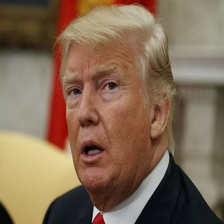
\includegraphics[height=5cm, width=\linewidth, keepaspectratio]{image0.jpg}
  \caption{The starting image}
\end{subfigure}
\begin{subfigure}{.5\textwidth}
  \centering
  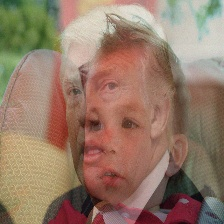
\includegraphics[height=5cm, width=\linewidth, keepaspectratio]{image1000.jpg}
  \caption{1000 queries}
\end{subfigure}

\begin{subfigure}{.5\textwidth}
  \centering
  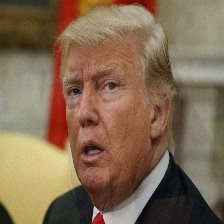
\includegraphics[height=5cm, width=\linewidth, keepaspectratio]{image2000.jpg}
  \caption{2000 queries}
\end{subfigure}
\begin{subfigure}{.5\textwidth}
  \centering
  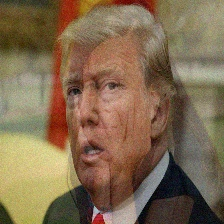
\includegraphics[height=5cm, width=\linewidth, keepaspectratio]{image4000.jpg}
  \caption{4000 queries}
\end{subfigure}

\begin{subfigure}{.5\textwidth}
  \centering
  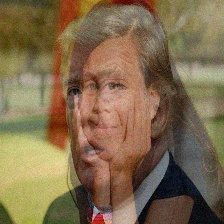
\includegraphics[height=5cm, width=\linewidth, keepaspectratio]{image8000.jpg}
  \caption{8000 queries}
\end{subfigure}
\begin{subfigure}{.5\textwidth}
  \centering
  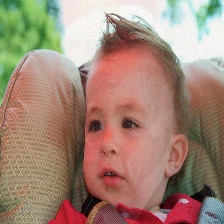
\includegraphics[height=5cm, width=\linewidth, keepaspectratio]{image12000.jpg}
  \caption{12000 queries}
\end{subfigure}

\begin{subfigure}{.5\textwidth}
  \centering
  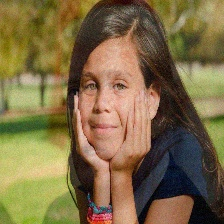
\includegraphics[height=5cm, width=\linewidth, keepaspectratio]{image16000.jpg}
  \caption{16000 queries}
\end{subfigure}
\begin{subfigure}{.5\textwidth}
  \centering
  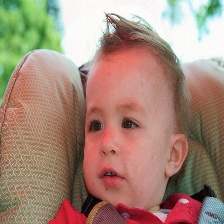
\includegraphics[height=5cm, width=\linewidth, keepaspectratio]{final_adversarial.jpg}
  \caption{Final adversarial sample}
\end{subfigure}
\caption{Although an adversary is changing the image, the blackbox classifier is not changing the prediction (68 years old)}
\label{fig:trump-adv}
\end{figure}

\begin{figure}
\begin{subfigure}{.5\textwidth}
  \centering
  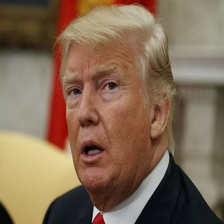
\includegraphics[height=5cm, width=\linewidth, keepaspectratio]{image0.jpg}
  \caption{Starting image}
\end{subfigure}
\begin{subfigure}{.5\textwidth}
  \centering
  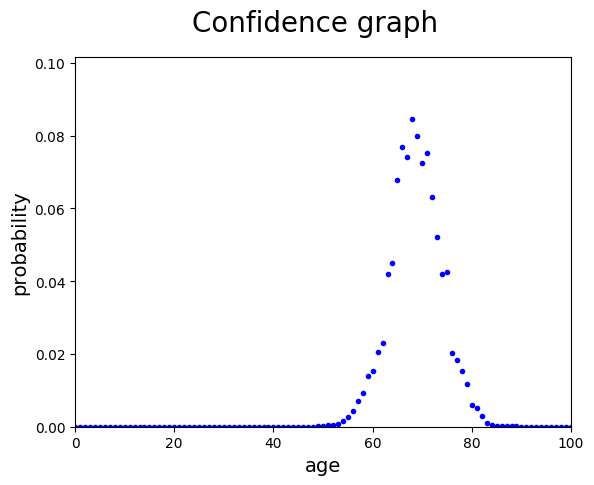
\includegraphics[height=5cm, width=\linewidth, keepaspectratio]{softmaxbenign.png}
  \caption{Predictions for the starting image}
\end{subfigure}
\caption{Starting image and the corresponding prediction}
\label{fig:starting-image-softmax}
\end{figure}

\begin{figure}
\begin{subfigure}{.5\textwidth}
  \centering
  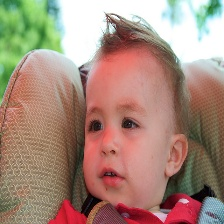
\includegraphics[height=5cm, width=\linewidth, keepaspectratio]{source_image.jpg}
  \caption{The targeted image}
\end{subfigure}
\begin{subfigure}{.5\textwidth}
  \centering
  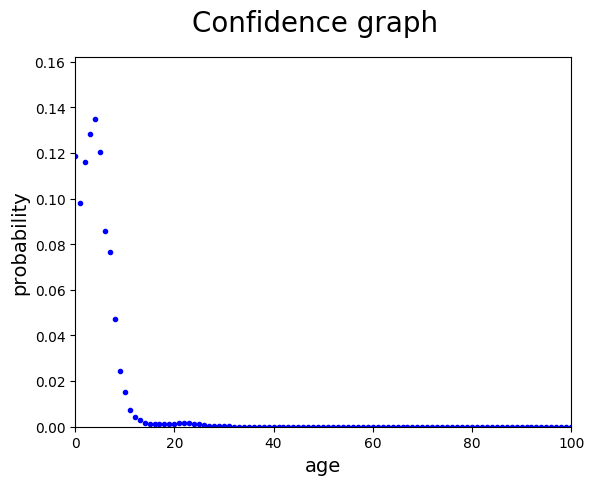
\includegraphics[height=5cm, width=\linewidth, keepaspectratio]{softmaxsource_image.png}
  \caption{Predictions for the targeted image}
\end{subfigure}

\caption{Targeted image and the corresponding predictions}
\label{fig:targeted-image-softmax}
\end{figure}

\begin{figure}

\begin{subfigure}{.5\textwidth}
  \centering%
  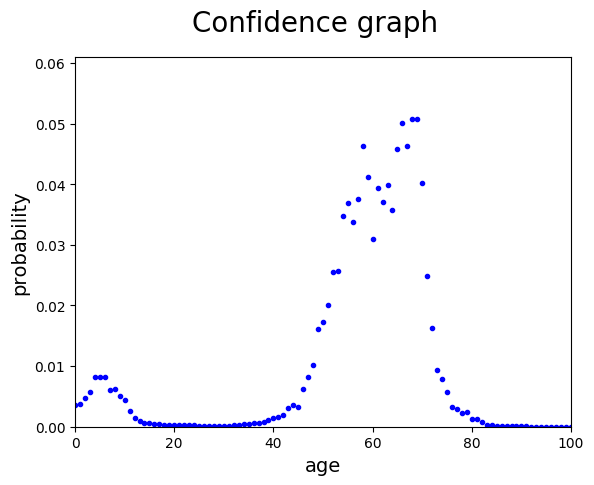
\includegraphics[height=5cm, width=\linewidth, keepaspectratio]{softmax3000.png}
  \caption{3000 queries}
\end{subfigure}
\begin{subfigure}{.5\textwidth}
  \centering%
  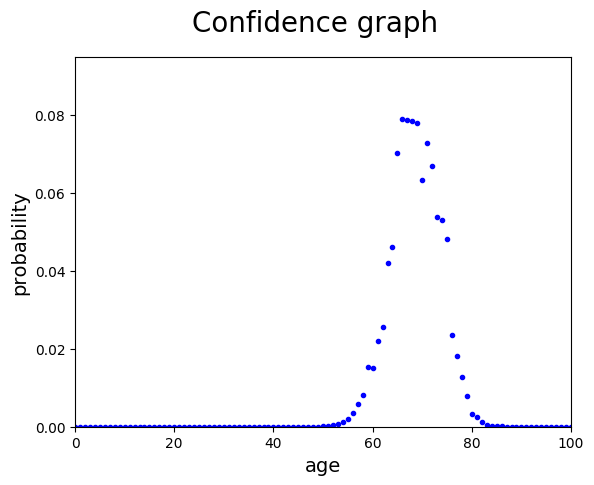
\includegraphics[height=5cm, width=\linewidth, keepaspectratio]{softmax4000.png}
  \caption{4000 queries}
\end{subfigure}


\begin{subfigure}{.5\textwidth}
  \centering%
  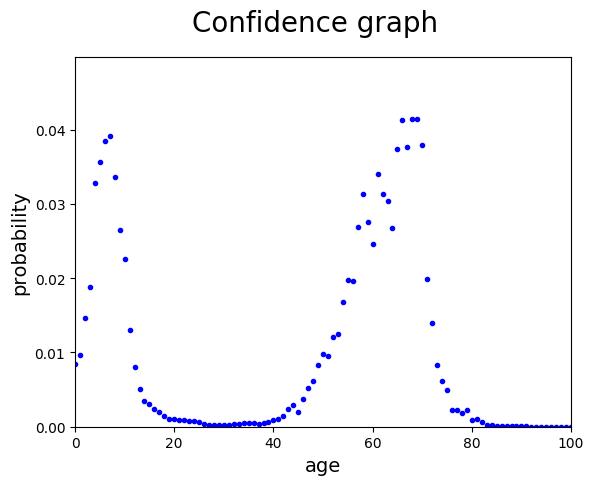
\includegraphics[height=5cm, width=\linewidth, keepaspectratio]{softmax8000.png}
  \caption{8000 queries}
\end{subfigure}
\begin{subfigure}{.5\textwidth}
  \centering%
  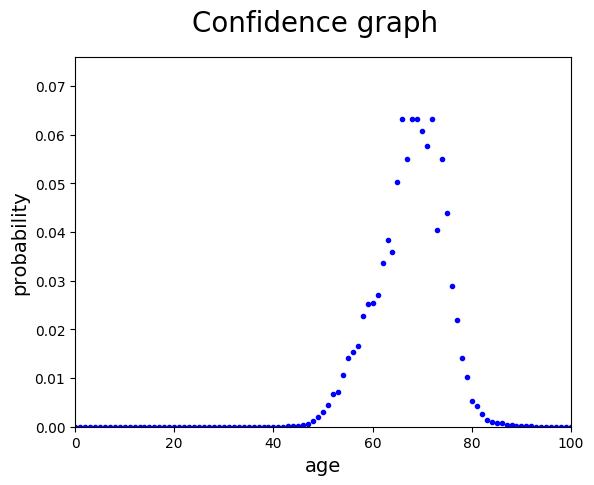
\includegraphics[height=5cm, width=\linewidth, keepaspectratio]{softmaxadversarial.png}
  \caption{The final adversarial sample (77 000 queries)}
\end{subfigure}

\caption{Predictions of the blackbox classifier for images corresponding to Figure \ref{fig:trump-adv}. In all the graphs, age 68 is predicted with the maximum probability.}
\label{fig:trump-softmax}
\end{figure}


